\begin{figure}[tbp]
\begin{center}
\includegraphics[width=0.48\textwidth]{cl_correlation_z1_z2.eps}
\end{center}
\vspace{-0.7cm}
\caption{The cross correlation r between reconstructed kSZ $P_{\hat \Theta_{kSZ}}$ 
and real kSZ $P_{\Theta_{kSZ}}$.
    (Dashed line) kSZ calculated from foreground substracted 21cm density field $\delta_{fs}$;
    (Solid line) kSZ calculated from tidal reconstructed density field.
    (Blue lines) take into account of redshift distortions.
}
\label{fig:r}
\end{figure}
1. Correlation of reconstructed velocity fields: 

We first present the result about reconstructed velocity field(Eq.(\ref{eq:v})) in Fig.\ref{fig:v}.
The upper two panels show the cross correlation r between $v_z$ and 
$\hat v_z^{fs}$ calculated from foreground substracted field $\delta_{fs}$; 
the lower panel shows the cross correlation between $v_z$ and $\hat v_z^{tide}$ calculated from $\hat \kappa_c$. 
The contour line represent the value of $k^3 P(k)$, which is related to the importance of each mode when generating kSZ signals.

Notice: 1. Although the foreground at z=2 is stronger, 
the non-linear effects are weaker.  
Therefore, we can still see some correlations at $k\parallel \lesssim 0.1$, with the little density signals left. 
And these correlations are even better than the z=1 case after the gaussianization.

On the other hand, there is degrading performance of tidal reconstruction on z=2. 
This is likely due to the stricter cutoff $k_c=0.32 h/Mpc$ compared to $k_c=0.5 h/Mpc$ at z=1.

2. Since tidal reconstruction relies strongly on large k modes, and we only lost small $k_z$ modes in the foreground(Fig.\ref{fig:v} upper panel). 
The reconstruction on $k_\parallel$ is better than on $k_\perp$, which is an advantage for estimating $v_z$.

Important to see: 
1. The previously lost small $k_\parallel$ modes has been well reconstructed through the 3D tidal reconstruction procedures. 
2. The modes recovered in tidal reconstruction play more vital role in generating kSZ signals. 

2. Correlation of reconstructed kSZ signals:

In Fig.\ref{fig:r}, 
we demonstrate the correlation r between the reconstructed kSZ signal $\hat \Theta$ and original kSZ signal $\Theta$ (black lines). 
We used both orginal foreground substracted density field and tidal reconstructed density field and compare the different results. 

Important to see:
1. For z=1, there are significant improvement on the cross-correlation after tidal reconstruction, especially below $l\sim 2000$
2. For z=2, the tidal reconstruction improves the cross-correlation for $l\lesssim 800$. 
However, since the non-linear effect is less strong at this stage, 
the orginal 21cm density field is good enough to reconstruct kSZ signal for $l \gtrsim 800$. 
Combining them, we would have good cross-correlation for $l \sim 20-8000$.

In all, for both redshift, with the non-ideal foregrounds and resolutions we assume, 
we are able to obtain a correlation $r \gtrsim 0.5$ for $l\sim 50-5000$ between 21cm density field and kSZ signals.

